%\section{Understanding and Modeling Transient Server Preemptions}
%\section{Modeling the Dynamics of Transient Server Preemptions}
\section{Preemption Dynamics of Transient Cloud Servers}

%Understanding the nature and dynamics of transient cloud servers such as their preemption frequency is a prerequisite to understand and improve the performance of applications.

In order to understand and improve the performance of applications running on transient cloud servers, we must understand the nature and dynamics of their preemptions.
The preemption characteristics are governed by the supply of surplus resources, the demand for cloud resources, and the resource allocation policies enforced by the cloud operator.
Therefore, in this section, we present empirical and analytical models to help us understand the nature of preemptions. 



% Transient cloud servers, by their very nature have limited availability and are frequently preempted.
% These preemptions are akin to fail-stop failures, and are often preceeded by a small advance warning (few seconds) to allow for graceful shutdowns.

% Since preemptions can impact the availability, performance, and cost of running applications, in this section, we examine their preemption characteristics.
% This modeling is important, because having a model of the availability can be useful in the context of predicting the running times of applications.
% Cloud providers offer a large number of servers of different configurations and types.
% Since transient server availability is fundamentally tied to supply and demand, the availability of servers of different types can be significantly different. 
% Thus, selecting the ``right'' server type is crucial for minimizing the overall costs. 




\subsection{Price based preemption models}

Amazon's EC2 spot instances were the original cloud transient servers.
The preemptions of EC2 spot instances is based on their \emph{price}, which is dynamically adjusted based on the supply and demand of cloud resources.
Spot prices are determined based on a continuous second-price auction, and if the spot price increases above a pre-specified maximum-price, then the server is preempted.

Thus, the time-series of these spot prices can be used for understanding preemption characteristics such as the frequency of preemptions and the ``Mean Time To Failure'' of the spot instances.
Many research projects have used publicly available\footnotemark historical spot prices to characterize and model spot instance preemptions~\cite{spotcheck,how-to-bid}. %Add lots more here 
For example, past work has analyzed spot prices and shown that the MTTF's of spot instances of different hardware configurations and geographical zones ranges from a few hours to a few days~\cite{prateek-thesis, shastri-thesis}. 


\footnotetext{Amazon posts Spot prices of 3 months, and researchers have been collecting these prices since 2010~\cite{Buyya-prices}.}

However, Amazon has recently changed the preemption characteristics of spot instances, and servers are now preempted even if the spot price is below the maximum price.
Thus, spot prices are no longer a completely reliable indicator of preemptions, and preemptions can no longer be inferred from looking at prices alone.
Therefore, new techniques are required to model preemption dynamics that can supplement the earlier price-based approaches, and we develop these techniques next.

%\cite{alicloud-spot, packet-spot}

\subsection{Empirical preemption models}

The preemptions of transient servers need not be related to their price.
For example, Google's Preemptible VMs and Azure Batch VMs have a \emph{fixed} price relative to their non-preemptible counterparts. 
In such cases, price based models are inadequate, and other approaches to understand preemptions is required.

This task is further complicated by the fact that these cloud operators (Google and Microsoft) do not currently provide any information about preemption characteristics. 
Thus, relatively little is known about the preemptions (and hence the performance) of these transient VMs. %significantly limiting their use?

In order to understand preemption dynamics of transient servers, we conduct a large-scale empirical measurement study which is the first of its kind. 
We launched more than 1000 Google Preemptible VMs of different types over a two month period (Feb--April 2019), and measured their time to preemption (aka, their useful lifetime).\footnotemark

\footnotetext{We will release the complete preemption dataset and hope that other researchers can benefit.} %Weaksauce 


\begin{figure}
  \centering
  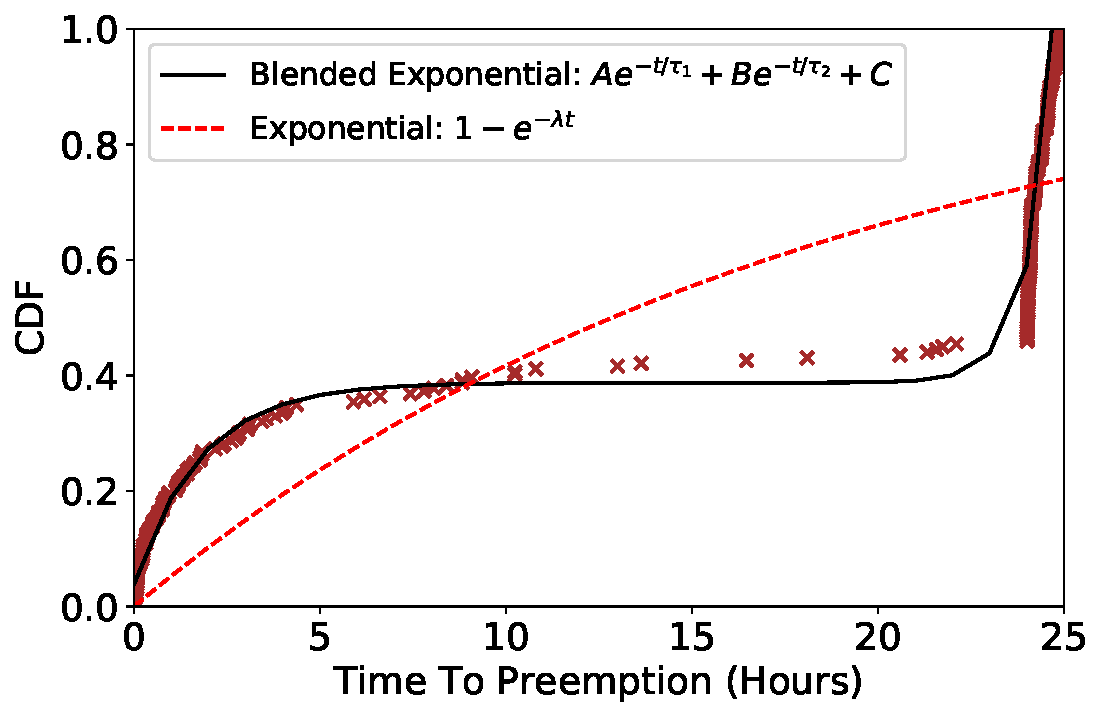
\includegraphics[width=0.4\textwidth]{../data/cdf_all.pdf}
  \caption{CDF of lifetimes of Google Preemptible Instances. Our blended exponential distribution fits much better than the conventional exponential failure distributions. }
  \label{fig:gcp1}
\end{figure}


A sample of 100 such preemption events are shown in Figure~\ref{fig:gcp1}, which shows cumulative distribution of the VM lifetimes. 
Note that the cloud operator (Google) caps the \emph{maximum} lifetime of the VM to 24 hours, and all the VMs are preempted before that hard limit.
Furthermore, the lifetimes of VM's are \emph{not} uniformly distributed, but have three distinct phases. 
We observe that many VM's are quickly preempted after they are launched, and thus have a steep rate of failure initially.
The failure rate is ``bath tub'' shaped, with VM's that survive past 3 hours enjoying a relatively low preemption rate, and finally a steep increase in the number of preemptions as the preemption deadline (24 hours) approaches. 


We note that this preemption behavior, imposed by the small, 24 hour  lifetime, is \emph{substantially} different from conventional failure characteristics of hardware components and even EC2 spot instances.
In these ``classical'' setups, the rate of failure is usually modeled using an exponential distribution, such that $f(t) = \lambda e^{-\lambda t}$, where $\lambda=1/\text{MTTF}$.
However, Figure~\ref{fig:gcp1} also shows the CDF ($=1-e^{-\lambda t}$) of the exponential distribution when fitted to the observed preemption data, by finding the distribution parameter $\lambda$ that minimizes the least squares error.
From Figure~\ref{fig:gcp1}, we can see that the classic exponential distribution is unable to model the observed preemption characteristics.
The primary reason is that the exponential distribution assumes that the preemptions are \emph{memoryless}, which does not hold true when there is a fixed upper bound on the lifetime, as is the case for Google Preemptible VMs.

\subsection{Analytical modeling of preemptions in Google cloud}

In order to better understand and characterize preemptions, we now develop a general analytical model for preemption dynamics that is faithful to the empirically observed data and that provides a basis for developing running-time and cost minimizing optimizations that we present in Section~\ref{sec:design}.


Our model is based on our earlier observation that the distribution of cumulative lifetimes has multiple distinct temporal phases.
In order to model the overall empirical CDF, we develop a \emph{new} probability distribution that is composed by blending two failure processes that act on different temporal phases over the 24 hour maximum lifetime of the VMs. 

We write the general form of our blended preemption CDF as follows:

\begin{equation}
  \label{eq:blend1}
  F_{\text{Blended}}(t) = A(1-e^{-t/\tau_1} + e^{\frac{t-b}{\tau_2}})
\end{equation}

For most of it's life, a VM sees failures according to the convential exponential distribution with a rate of failure equal to $1/\tau_1$, which is the first term in~\ref{eq:blend1}. 
However, this does not capture the finite lifetime of the VM imposed by the cloud operator.
As VMs get closer to their maximum lifetime (24 hours), they are reclaimed (i.e., preempted) at a high, exponential rate, which is captured in the second term of the CDF ($e^{\frac{t-b}{\tau_2}}$). 
However, this exponential reclamation is only applicable towards the end of the VM's maximum lifetime, and thus the $(t-b)$ term helps to ensure that it does not dominate over the entire temporal range.
As before, $1/\tau_2$ is the rate of the reclamation.

This ``blended exponential'' distribution thus captures the different phases of the preemption CDF through parameters $\tau_1, \tau_2, b$, and the parameter $A$ is used to ensure we meet the boundary conditions ($F(0)=0, F(24)=1$)
These parameters can be obtained for a given empirical CDF by minimizing least-squared function fitting methods. \footnotemark 

\footnotetext{More details about the distribution fitting are presented in the implementation section(~\ref{sec:impl}}


In the next section, we use the blended exponential analytical model for optimizing cloud resource selection such that we can run scientific applications at low cost and running times.


%%%%%%%%%%%%%%%%%%%% OPTIONAL


\textbf{Optional text. Spoils flow currently}
Preemption dynamics can also be analyzed through the \emph{survival rates} of VMs.
Let $S(t)$ denote the number of VMs that survive till time $t$.
Then, without loss of generality: $F(t) = A(1-S(t))$
% Well actually, not really. A spoils that, but whatevs.

In the case of the blended exponential distribution, $S(t)$ depends on $S(t)$ itself, as well as the failure rates of different phases and the current lifetime ($t$), as follows:
\begin{equation}
  \label{eq:ramanujan}
  \dfrac{dS(t)}{dt} = \{\dfrac{1}{\tau_2} - \dfrac{1}{\bar{\tau}}(\dfrac{1}{1-e^{-b/\tau_2} \cdot e^{t/\bar{\tau}}}) \}S(t)
\end{equation}



% \subsection{EC2 spot instances}

% The earliest form of transient cloud instances.
% In addition to having dynamic availability, also have dynamic pricing.
% ``Classic'' spot instances had price determining the availability, and thus a large amount of work was devoted to bidding and analyzing the prices.

% However a recent change to the spot prices no longer allows these assumptions, rendering it impossible to obtain the \emph{exact} availability information from the prices alone.


% \subsection{Google Preemptible VMs}

% Launched in 2015.
% Flat-rate discount of 80\% compared to on-demand servers.
% Interesting availability SLA: the maximum lifetime is 24 hours, and can be preempted earlier as well.

% In this paper we will look at these preemptible VMs and show how to model their availability.
% Given the inability to use EC2 prices, we believe that our approach is more generalizable and robust.


% There are some distinguishing characteristics of GCP preemptible VMs that makes their failure modeling challenging.
% First is their flat pricing and no other signalling information about their preemption rates (MTBFs) that makes server selection difficult.

% \textbf{Modeling Failure Behavior of Preemptible VMs}
% CDF is ``sigmoid'' shaped.
% $P=R*np.sinh((t-t0)/tau) + C$ with a very low $R=10^{-6}, t_0=12, \tau=0.9, C=0.36$

% Basically, this is a mixture of two distributions, the standard exponential distribution, which we call the stabilization rate and an exponentially increasing reclamation rate.

% Preemptible VMs have three availability phases.

% There are many early deaths, then a period of low failure rates, and then the failure rate is exponential with a positive exponent to enable the cloud provider to reclaim the VMs within the deadline (24 hours in the case of Google's Preemptible VMs).








%%% Local Variables:
%%% mode: latex
%%% TeX-master: "paper"
%%% End:
